\documentclass{article}

% if you need to pass options to natbib, use, e.g.:
\PassOptionsToPackage{numbers, compress}{natbib}
% before loading nips_2017
%
% to avoid loading the natbib package, add option nonatbib:
% \usepackage[nonatbib]{nips_2017}

\usepackage{nips_2018}

% to compile a camera-ready version, add the [final] option, e.g.:
% \usepackage[final]{nips_2017}

\usepackage[utf8]{inputenc} % allow utf-8 input
\usepackage[T1]{fontenc}    % use 8-bit T1 fonts
\usepackage{hyperref}       % hyperlinks
\usepackage{url}            % simple URL typesetting
\usepackage{booktabs}       % professional-quality tables
\usepackage{amsfonts}       % blackboard math symbols
\usepackage{nicefrac}       % compact symbols for 1/2, etc.
\usepackage{microtype}      % microtypography

\usepackage{hyperref}

\usepackage{amssymb}
\usepackage{xspace}

\usepackage{amsmath}

% For citations
\usepackage{natbib}

% For figures
\usepackage{graphicx} % more modern
\usepackage{wrapfig}
%\usepackage{epsfig} % less modern
%\usepackage{subfigure} 
\usepackage{subcaption}
\usepackage{multirow}
\usepackage{adjustbox}

\usepackage{listings}
\usepackage{textcomp}

% For assumptions
\usepackage{amsthm,amssymb,amsopn}
\newtheorem{assumption}{Assumption}
\newtheorem{define}{Definition}
\newtheorem{thm}{Theorem}
\newtheorem{lem}{Lemma}
\newtheorem{coro}{Corollary}
\newtheorem{condition}{Condition}

% For algorithms
\usepackage{algorithm}
\usepackage{algorithmic}
\renewcommand{\algorithmiccomment}[1]{~~~~\textcolor{gray}{$\triangleright$\textit{#1}}}
\renewcommand{\algorithmicrequire}{\textbf{Input:}}
\renewcommand{\algorithmicensure}{\textbf{Output:}}
\makeatletter
\makeatletter
\newcommand*{\da@rightarrow}{\mathchar"0\hexnumber@\symAMSa 4B }
\newcommand*{\da@leftarrow}{\mathchar"0\hexnumber@\symAMSa 4C }
\newcommand*{\xdashrightarrow}[2][]{%
  \mathrel{%
    \mathpalette{\da@xarrow{#1}{#2}{}\da@rightarrow{\,}{}}{}%
  }%
}
\newcommand{\xdashleftarrow}[2][]{%
  \mathrel{%
    \mathpalette{\da@xarrow{#1}{#2}\da@leftarrow{}{}{\,}}{}%
  }%
}
\newcommand*{\da@xarrow}[7]{%
  % #1: below
  % #2: above
  % #3: arrow left
  % #4: arrow right
  % #5: space left 
  % #6: space right
  % #7: math style 
  \sbox0{$\ifx#7\scriptstyle\scriptscriptstyle\else\scriptstyle\fi#5#1#6\m@th$}%
  \sbox2{$\ifx#7\scriptstyle\scriptscriptstyle\else\scriptstyle\fi#5#2#6\m@th$}%
  \sbox4{$#7\dabar@\m@th$}%
  \dimen@=\wd0 %
  \ifdim\wd2 >\dimen@
    \dimen@=\wd2 %   
  \fi
  \count@=2 %
  \def\da@bars{\dabar@\dabar@}%
  \@whiledim\count@\wd4<\dimen@\do{%
    \advance\count@\@ne
    \expandafter\def\expandafter\da@bars\expandafter{%
      \da@bars
      \dabar@ 
    }%
  }%  
  \mathrel{#3}%
  \mathrel{%   
    \mathop{\da@bars}\limits
    \ifx\\#1\\%
    \else
      _{\copy0}%
    \fi
    \ifx\\#2\\%
    \else
      ^{\copy2}%
    \fi
  }%   
  \mathrel{#4}%
}
\makeatother

% for todos
\usepackage{xargs}                      % Use more than one optional parameter in a new commands
\usepackage[pdftex,dvipsnames]{xcolor}
%todos -- remove at end
%\usepackage[colorinlistoftodos,prependcaption,textsize=tiny]{todonotes}
%\newcommand{\unsure}[2][1=]{\todo[disable,linecolor=red,backgroundcolor=red!25,bordercolor=red,#1]{#2}}
%\newcommand{\change}[2][1=]{\todo[disable,linecolor=blue,backgroundcolor=blue!25,bordercolor=blue,#1]{#2}}
%\newcommand{\info}[2][1=]{\todo[disable,linecolor=OliveGreen,backgroundcolor=OliveGreen!25,bordercolor=OliveGreen,#1]{#2}}
%\newcommand{\improvement}[2][1=]{\todo[disable,linecolor=Plum,backgroundcolor=Plum!25,bordercolor=Plum,#1]{#2}}

% quick-and-dirty TKTKTK
\newcommand{\highlight}[1]{\colorbox{yellow}{#1}}


\title{Supplementary Material for Predicting Electron Paths}

% The \author macro works with any number of authors. There are two
% commands used to separate the names and addresses of multiple
% authors: \And and \AND.
%
% Using \And between authors leaves it to LaTeX to determine where to
% break the lines. Using \AND forces a line break at that point. So,
% if LaTeX puts 3 of 4 authors names on the first line, and the last
% on the second line, try using \AND instead of \And before the third
% author name.

\author{
  David S.~Hippocampus\thanks{Use footnote for providing further
    information about author (webpage, alternative
    address)---\emph{not} for acknowledging funding agencies.} \\
  Department of Computer Science\\
  Cranberry-Lemon University\\
  Pittsburgh, PA 15213 \\
  \texttt{hippo@cs.cranberry-lemon.edu} \\
  %% examples of more authors
  %% \And
  %% Coauthor \\
  %% Affiliation \\
  %% Address \\
  %% \texttt{email} \\
  %% \AND
  %% Coauthor \\
  %% Affiliation \\
  %% Address \\
  %% \texttt{email} \\
  %% \And
  %% Coauthor \\
  %% Affiliation \\
  %% Address \\
  %% \texttt{email} \\
  %% \And
  %% Coauthor \\
  %% Affiliation \\
  %% Address \\
  %% \texttt{email} \\
}

\newcommand{\xb}{\mathbf{x}}
\newcommand{\Xc}{\mathcal{X}}
\newcommand{\Zc}{{\mathcal{Z}}}
\newcommand{\Mc}{{\mathcal{M}}}
\newcommand{\Bc}{{\mathcal{B}}}
\newcommand{\Ac}{{\mathcal{A}}}
\newcommand{\Pc}{{\mathcal{P}}}
\newcommand{\bb}{{\mathbf{b}}}
\newcommand{\ab}{{\mathbf{a}}}
\newcommand{\mb}{{\mathbf{m}}}
\newcommand{\Mb}{{\mathbf{M}}}
\newcommand{\Pb}{{\mathbf{P}}}
\newcommand{\Hb}{{\mathbf{H}}}
\newcommand{\Ab}{{\mathbf{A}}}
\newcommand{\Rc}{{\mathcal{R}}}
\newcommand{\delb}{{\boldmath{\delta}}}


%
\newcommand{\nodeEmbeddings}[1]{\Hb_{#1}}
\newcommand{\graphEmbeddings}{\mathbf{h_g}}
%\newcommand{\graph}{\mathcal{G}}



\newcommand{\actionLogits}{\textbf{s}} % for nodes

% The model definitions
\newcommand{\electronPath}{\Pc}
\newcommand{\moleculeSet}{\Mc}
\newcommand{\initialAndReactants}{\Mc_0, \Mc_r}

\newcommand{\contextVect}{\bm{c}}
% Then the modules!
\newcommand{\fEmbed}{g_{\Ac}} % for nodes
\newcommand{\fEmbedGraphs}{r} % for nodes


\newcommand{\fAdd}{f_{\textrm{add}}}
\newcommand{\fRemove}{f_{\textrm{remove}}}
\newcommand{\fInitial}{f_{\textrm{initial}}}
\newcommand{\fStop}{f_{\textrm{stop}}}
\newcommand{\fReagEmbed}{f_{\textrm{reagent}}}
\newcommand{\fModules}{\fEmbed, \fAdd, \fRemove, \fInitial,\fStop, \fReagEmbed}
\newcommand{\fui}{f_i}
\newcommand{\fuj}{f_j}
\newcommand{\fuk}{f_k}
\newcommand{\fum}{f_m}

\newcommand{\actionProb}[2][]{ p(a_{#2} \mid \moleculeSet_{\electronPath_{0:#2-1}^{#1}}, a^{#1}_{#2-1}, #2)}
\newcommand{\continueProb}[2]{p(s_{#1}' \mid \moleculeSet_{#2}) }


\begin{document}
\maketitle


\section{Example of symmetry affecting evaluation of electron paths}
In the main text we described the challenges of how to evaluate our model, as different electron paths can form the same products, for instance due to symmetry.
Figure \ref{fig:symmetric-reaction-example} is an example of this.


\begin{figure*}[h]

    \centering
    \begin{subfigure}[b]{0.95\textwidth}
        \centering
        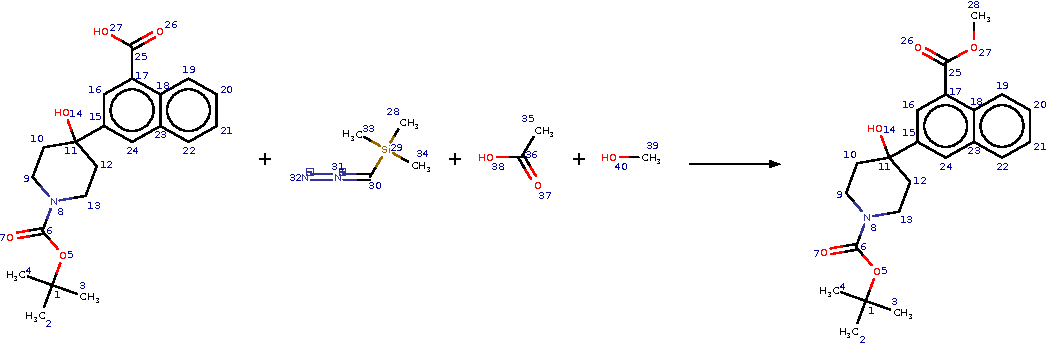
\includegraphics[height=1.2in]{imgs/reaction}
        \caption{Reaction as defined by USPTO SMILES}
    \end{subfigure}
    
    \par\bigskip % force a bit of vertical whitespace 
    \begin{subfigure}[b]{0.95\textwidth}
        \centering
        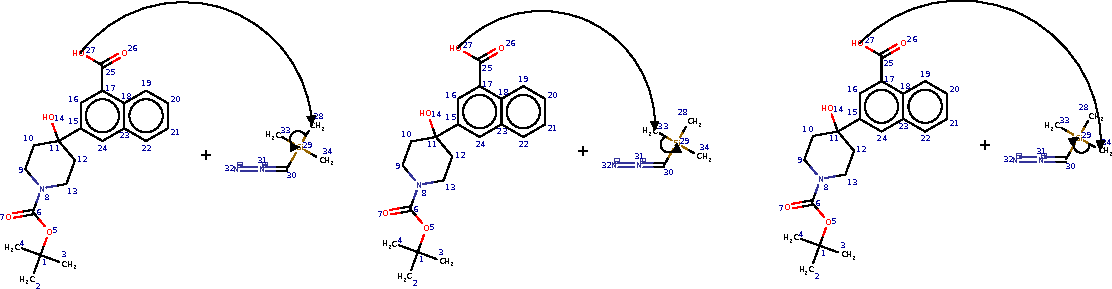
\includegraphics[height=1.2in]{imgs/routes}
        \caption{Possible action sequences that all result in same major product.}
    \end{subfigure}
    \caption{This example shows how symmetry can affect the evaluation of electron paths. In this example, although one electron path is given in the USPTO dataset, after the O (atom map number 27) loses its Hydrogen it can react with any of the CH3 groups in the second reactant to form the same major product. This is why judging purely based on electron path accuracy can sometimes be misleading.}
    \label{fig:symmetric-reaction-example}
\end{figure*}


\section{More training details}

In this section we go through more specific model architecture details omitted from the main text. Further details can be found from our code, available at REDACTED.


\subsection{Model architectures}
In this section we provide further details of our model architectures.

Section 3 of the main paper discusses our model.
In particular we are interested in computing three conditional probability terms: (1) $p_\theta(a_0 \mid \initialAndReactants)$, the probability of the initial state $a_0$ given the reactants and reagents; 
(2) the conditional probability $p_\theta(a_t \mid a_{t-1}, \moleculeSet_t, t)$ 
%\todo[]{maybe somehow refer to "bond type" instead of $t$?} 
of next state $a_t$ given the intermediate products $\moleculeSet_t$ for $t > 0$;
and (3) the probability $p_\theta(s_t \mid \moleculeSet_t)$ that the reaction terminates with final product $\moleculeSet_{t}$.

Each of these is parametrized by NNs. We can split up the components of these NNs into a series of modules, all introduced in the main text: $\fEmbed$, $\fEmbedGraphs_{\textrm{stop}}$, $\fEmbedGraphs_\mathrm{reagent}$, $\fAdd$, $\fRemove$ and $\fInitial$.
 In this section we shall go through each of these in turn.

The function $\fEmbed$ computes node embeddings, $\nodeEmbeddings{\moleculeSet_t}$, which are used as input to all the other modules. For this we use Gated Graph Neural Networks (GGNN) \citep{li2016gated, gilmer2017neural}.
 We use 4 propagation steps. 
 The atom features we feed in are detailed in Table \ref{table:atom-features}. These are calculated using RDKit. In total there are 101 features and we maintain this dimensionality in the hidden layers during the propagation steps of the GGNN. Three edge labels are defined: single bonds, double bonds and triple bonds. RDKit is used to Kekulize the reactant molecules. 

\begin{table}
  \caption{Atom features}
  \label{table:atom-features}
  \centering
  \begin{tabular}{ll}
    \toprule
    Feature     & Description      \\
    \midrule
    Atom type & 72 possible elements in total, one hot  \\
    Degree     & One hot (0,   1,   2,   3,   4,   5,   6,   7,  10)  \\
    Explicit Valence     & One hot   (0,   1,   2,   3,   4,   5,   6,   7,   8,  10,  12,  14)    \\
    Hybridization & One hot (SP, SP2, SP3, Other) \\
    H count & integer \\
    Electronegativity & float \\
    Atomic number & integer \\
    Part of an aromatic ring & boolean\\
    \bottomrule
  \end{tabular}
\end{table}

As mentioned in Section 3 of the main paper both $\fEmbedGraphs_{\textrm{stop}}$, $\fEmbedGraphs_\mathrm{reagent}$ consist of three
linear functions. 
For  both the function $\fui$ is used to decide how much each node should contribute towards the embedding and so projects down to a scalar value.
Again for both, $\fuj$ projects the node embedding up to a higher dimensional space, which we choose to be 202 dimensions. 
This is double the dimension of the node features, and similar to the approach taken by \citet[\S B.1]{li2018learning}.
Finally, $\fuk$ differs between the two modules, as for $\fEmbedGraphs_{\textrm{stop}}$ it projects down to one dimension (to later go through a sigmoid function and compute a stop probability), whereas for  $\fEmbedGraphs_\mathrm{reagent}$, $\fuk$ projects  to a dimensionality of 100 to form the reagent embedding.


The modules for $\fAdd$ and $\fRemove$, that operate on each node to produce a action logit, are both NNs consisting of one hidden layer of 100 units. 
Concatenated onto the node features going into these networks are the node features belonging to the previous atom in the path.



The final function, $\fInitial$, is represented by an NN with hidden layers of 100 units. 
When conditioning on reagents (ie for
 \ourModelR
 )
  the reagent embeddings calculated by $\fReagEmbed$ are concatenated onto the node embeddings and we use two hidden layers for our NN. When ignoring reagents (ie for \ourModelIR) we use one hidden layer for this network. In total \ourModelR has approximately 250 000 parameters and \ourModelIR has approximately 190 000.

\subsection{Training}

We train everything using ADAM \citep{kingma2014adam} and an initial learning rate of 0.0001, which we decay after 5 and 9 epochs by a factor of 0.1. 
We train for a total of 10 epochs.
For training we use reaction minibatch sizes of one, although these can consist of multiple intermediate graphs.









\section{Prediction using our model}

At predict time, as discussed in the main text, we use beam search to find high probable chemically-valid paths from our model. Further details are given in Algorithm~\ref{algo:valid_path}.



\newcommand{\cProbCont}{\texttt{calc\_prob\_continue}}
\newcommand{\cProbAct}{\texttt{calc\_prob\_action}}
\newcommand{\cProbInitial}{\texttt{calc\_prob\_initial}}
\newcommand{\removeFlag}{F_\textrm{remove}}

\newcommand{\outputPool}{\hat{\Pc}}
\newcommand{\cPath}{\rho}
\newcommand{\lProb}{p_{\textrm{path}}}


%\begin{wrapfigure}{R}{0.5\textwidth}
\begin{figure}
\begin{minipage}{1.\textwidth}
\begin{algorithm}[H]
  \caption{Predicting electron paths at test time.}
  {\bf Input:}~~Molecule $\Mc_0$ (consisting of atoms $\Ac$), reagents $\Mc_r$ , beam width $K$, time steps $T^\mathrm{max}$
  
  \begin{algorithmic}[1]
  	% Set up pool of completed paths to sort later
  	\STATE $\outputPool = \{\left( \emptyset, \log (1 - \cProbCont(\Mc_0)) \right) \}$  \COMMENT{This set will store all completed paths.}
  	\STATE $\removeFlag \!=\!1$ \COMMENT{remove flag}
  	
  	% Pick the first action.\\
  	\STATE
	\STATE $\hat{\Bc} = \emptyset$.  \COMMENT{This set will store all possible open paths. Cleared at start of each timestep.}	
	\FORALL{$v \in \Ac$} 
		\STATE $ \cPath = (v)$
		\STATE $ \lProb = \log \cProbCont(\Mc_0) + \log \cProbInitial(v, \moleculeSet_0, \moleculeSet_r)$
		\STATE $\hat{\Bc} = \hat{\Bc} \cup \{\left(\cPath, \lProb \right)\}$
	\ENDFOR
	\STATE  $\Bc_{0} = \texttt{pick\_topK\_actions}(\hat{\Bc})$ \COMMENT{We filter down to the top K most promising actions.}
	
	% Then we evaluate the next stages.
	\STATE
	\FOR{t in $(1, \ldots, T^\mathrm{max})$}
		\STATE $\hat{\Bc} = \emptyset $ 
				
		% We take all the previous top K open paths from the previous step...
		\FORALL{$(\cPath, \lProb) \in \Bc_{t-1}$} 
			
			% We evaluate their stop probability at that point and add these stopped version to the completed pool.
			\STATE $\Mc_\cPath = \texttt{calc\_intermediate\_mol}(\Mc_0, \cPath)$
			\STATE $p_c = \cProbCont(\Mc_\cPath)$
			\STATE $\hat{\Pc} = \hat{\Pc} \cup \{(\cPath, \lProb + \log (1 - p_c))\}$
			
			% We then see what would happen if we continued and picked another action.
			\FORALL{$v \in \Ac$}
				\STATE $\cPath' = \cPath^\frown (v)$ \COMMENT{New proposed path is concatenation of old path with new node.}

				\STATE $v_{t-1} = $ last element of $\cPath$
				\STATE $\hat{\Bc} = \hat{\Bc} \cup \{(\cPath' , \lProb + \log p_c + \log \cProbAct(v, \Mc_\cPath, v_{t-1}, \removeFlag) )\}$
			\ENDFOR
		\ENDFOR
		
		% We next prune down the search space for next iteration to our beam width.
		\STATE  $\Bc_{t} = \texttt{pick\_topK\_actions}(\hat{\Bc})$ 
		
		% We indicate that the next step will be opposite step:
		\STATE $\removeFlag = \removeFlag + 1 \mod 2$. \COMMENT{If on add step change to remove and vice versa.}
	\ENDFOR
	
  % Finally we sort the pool and we are done
  \STATE
  \STATE $\outputPool = \texttt{sort\_on\_prob}(\outputPool)$
  \end{algorithmic}
  {\bf Output:}~~Valid completed paths and their respective probabilities, sorted by the latter, ~$\outputPool$
  \label{algo:valid_path}
\end{algorithm}
\end{minipage}
%\end{wrapfigure}
\end{figure}

\section{Further example of actions proposed by our model}

Figure \ref{fig:extra-textbook-example} shows the model's predictions for the mechanism of how two molecules will react. 

\begin{figure*}[h]
        \centering
        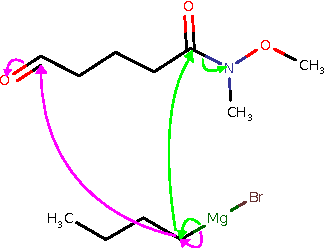
\includegraphics{imgs/textbook/reactants2}
        \caption{Predicted mechanism of our model on reactant molecules. Green arrow shows preferred mechanism, whereas pink shows the model's second preferred choice. Here, the top1 prediction is incorrect, but chemically reasonable. It should be rank2 instead.}
        \label{fig:extra-textbook-example}
\end{figure*}


\bibliography{bibliography}
\bibliographystyle{plainnat}
\end{document}

 